% TODO: should this be reduced?\
\chapter{System Integration}


\begin{figure}[h]
    \setlength{\abovecaptionskip}{5pt}    % Reduces space above caption
    \setlength{\belowcaptionskip}{5pt}    % Reduces space below caption
    \centering
    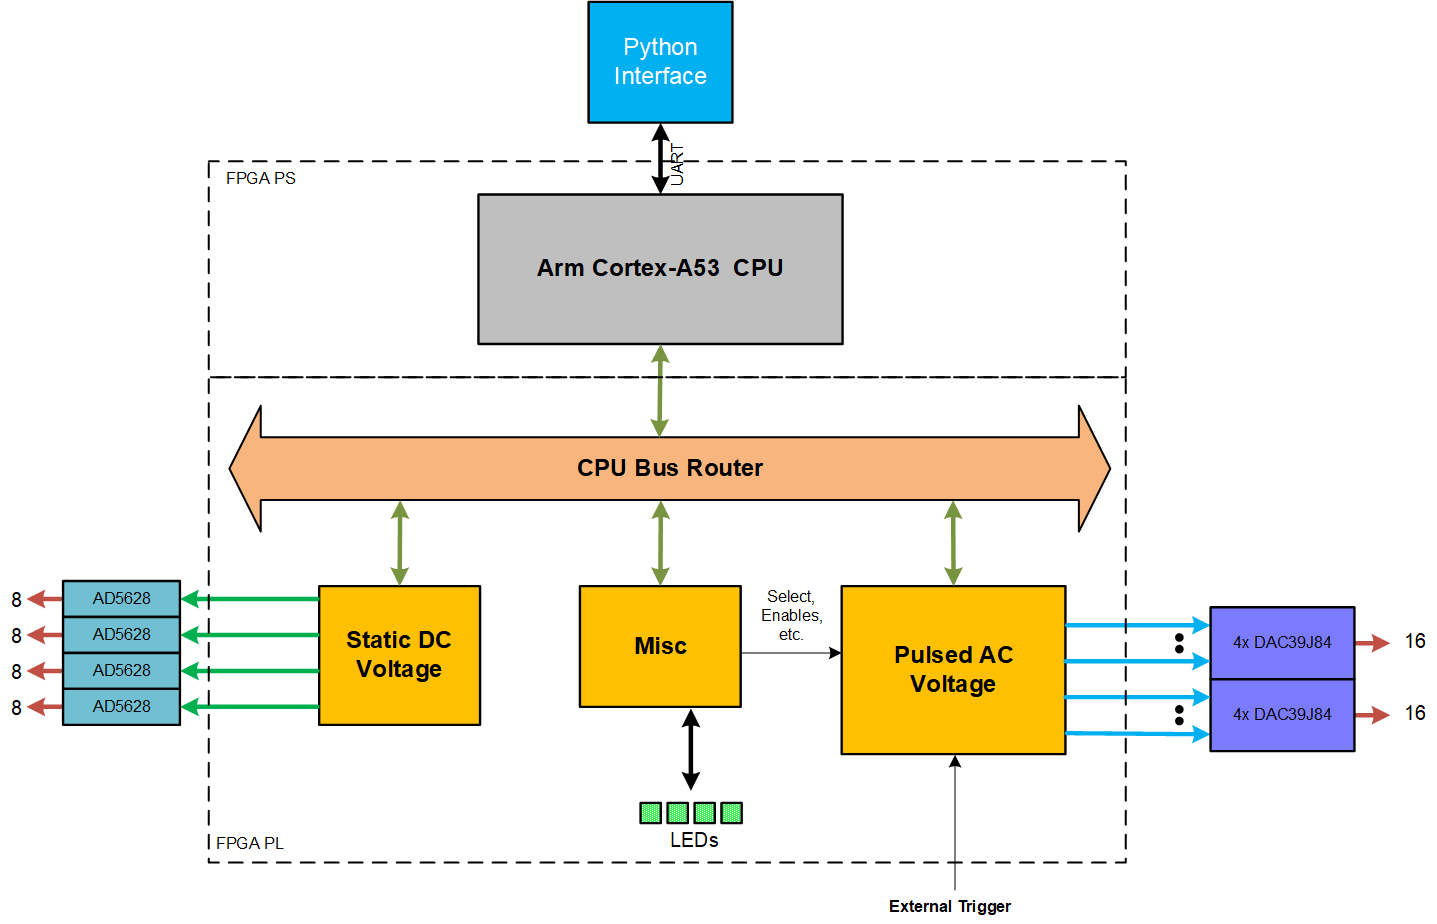
\includegraphics[width=1\linewidth]{figures/5.1.png}
    \caption{FPGA system architecture block diagram.}
    \label{fig:sys_diagram}
\end{figure}

The pulse channel module is an integral component of an FPGA system designed to generate 32 pulsed AC voltage signals and 32 static voltage signals. This system leverages both the processing systems and the programmable logic of the ZCU102 architecture. A Python-based interface allows users to input specific information about the pulses and voltage signals. This interface translates user requests into custom commands, which are then sent to the processing system via the FPGA's UART interface.

The processing system's ARM-based CPU converts Python-generated commands into addressable instructions for the FPGA's blocks. Within the FPGA hardware, a bus router takes the byte-addressable data from the CPU and translates it into block-specific word-addressable data. The system comprises three distinct hardware blocks, each serving a separate function. The orange blocks in \autoref{fig:sys_diagram} illustrate the names of these blocks, which will be discussed in detail in the subsequent sections. This architecture ensures efficient communication and data processing within the FPGA system, enhancing its overall performance and reliability.

% % TODO: this section is more translate Geoff to UW... does it rly needed to be mentioned in the thesis?
% \section{CPU Bus Router}

% The system utilizes a CPU interface adapter to bridge between the PS and the PL. This adapter plays a crucial role by converting byte-addressed signals from the PS AXI bus into a 32-bit word-addressed bus, which is essential for the proper functioning of the blocks within the FPGA design. Illustrated in \autoref{table:ps_addr}, the portions of the PS address are decoded into block select to choose one of the three available blocks in the system. Once a block is selected, the lower bits of the address are used to either write to or read from the chosen block. This ensures precise and efficient communication between the PS and the selected block. Additionally, a standardized register interface is implemented in each block to provide consistent access for control and status monitoring, thereby enhancing the system's reliability and ease of use. By employing this CPU interface adapter, the system achieves seamless integration between the PS and PL, facilitating efficient data transfer and control across the FPGA design. This design choice not only simplifies the communication process but also ensures scalability and flexibility for future enhancements.

 
% % TODO: explain more on this
% \begin{table}
% \centering
% \caption{Address convert format}
% 
\includegraphics[width=1.0\textwidth]{figures/pc_address.png}
% \label{table:ps_addr}
% \end{table}

\section{Static DC Voltage Block}
% TODO: replace with a clear picture
\begin{figure}[h]
    \setlength{\abovecaptionskip}{5pt}    % Reduces space above caption
    \setlength{\belowcaptionskip}{5pt}    % Reduces space below caption
    \centering
    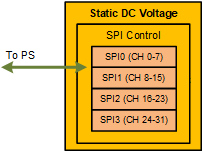
\includegraphics[width=0.5\linewidth]{figures/5.2.png}
    \caption{Block diagram for the DC voltage module}
    \label{fig:dc}
\end{figure}
The DC block provides stable and programmable static voltage control using four Analog Device AD5286 PMOD DACs. Each DAC supports eight voltage channels, making a total of 32 channels, as illustrated in \autoref{fig:dc}. Communication between the DACs and the system occurs via the SPI interface. These SPI interfaces are implemented as separate modules, each managing the clock, data, and chip select signals for data transmission to the DACs.

% TODO: Again... latex is not great for hardware so far...
\begin{table}[h]
\centering
\setlength{\abovecaptionskip}{5pt}    % Reduces space above caption
\setlength{\belowcaptionskip}{5pt}    % Reduces space below caption
\caption{SPI DAC message format}


\includegraphics[width=1.0\textwidth]{figures/spi_addr.png}
\label{table:spi_addr}
\end{table}

% Upon selection, the DC block converts part of the address and the lower 12-bit data from the processing system into SPI command as defined in \autoref{table:spi_addr}. 
The DC block utilizes the lower five bits of the CPU address to select one of four SPI-based DACs. Part of the address is used in the SPI message for the chosen DAC, as detailed in \autoref{table:spi_addr}. This address segment specifies the "channel select" portion of the command, determining which of the eight channels on the selected DAC will be used. The SPI message also includes an "update DAC" command to instruct the DAC to refresh the chosen channel's value, which is set in the "data" portion of the message. The processing system provides a 12-bit positive integer value for the DACs, which is then converted to a voltage value as specified by:

\begin{equation}
V_{out} = V_{ref} \times \frac{D}{2^{12}}
\end{equation}

Where $V_{out}$ is the voltage output by the DAC, $V_{ref}$ is the DAC's reference voltage, and $D$ is the data from the processing system \cite{ad5628}. This design ensures precise and flexible static voltage control. Additionally, the module supports write operations to update DAC channels and control features such as internal reference voltage and power. It also supports read operations, which return status flags for each SPI transaction. The use of multiple DACs and independent SPI modules allows for efficient handling of numerous voltage channels, providing enhanced control and reliability.

\section{Pulse AC Voltage Block}

The pulse generation module—also referred to as the AC block—is a synchronous multi-channel pulse generator designed to deliver precise control for laser operations on the photonic chips. Its architecture generates pulse sequences with a 10-nanosecond resolution across 32 channels, ensuring that each digital output is synchronized. 

\begin{figure}[h]
    \setlength{\abovecaptionskip}{5pt}    % Reduces space above caption
    \setlength{\belowcaptionskip}{5pt}    % Reduces space below caption
    \centering
    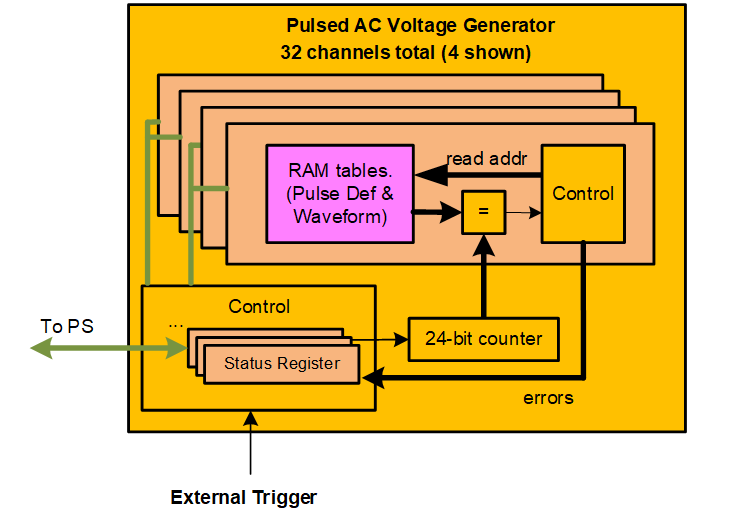
\includegraphics[width=0.8\linewidth]{figures/5.3.png}
    \caption{Block Diagram of the AC block.}
    \label{fig:george}
\end{figure}
The AC block acts as the central coordinator for all pulse channels. A Central Coordinator Process (CC-P) manages both external control signals and error notifications from individual channels, ensuring reliable overall performance. Central to its operation is a 24-bit counter that functions as a common timer, as seen in \autoref{fig:george}. Upon receiving an external trigger, this counter initiates the timing process uniformly for all channels. It continues until it reaches either a user-defined sequence length or its maximum value, at which point it sends stop signals to halt pulse generation. This coordinated stopping mechanism maintains timing precision and prevents runaway pulses that could lead to data inconsistencies.

A series of internal registers underpin the module's functionality. These registers store key parameters such as the total sequence length, the active channel enable, and select for memory reading and writing operations. Values are loaded into these registers via the CPU interface, which streams configuration data from the processing system. The design supports simultaneous writing to multiple channels, a useful feature for updating pulse parameters in parallel. However, because the data bus is only 32 bits wide, the system limits read operations to one channel at a time.

The module also incorporates an addressing scheme that distinguishes between channel-specific memory and internal control registers. The lower address range is reserved for waveform data and pulse parameters, while the upper range is dedicated to registers for the CC-P. Registers for settings such as sequence length, channel enables, and channel selections are both readable and writable. This bidirectional access permits real-time control and monitoring of each channel, facilitating adjustments as operational conditions change. In contrast, dedicated read-only registers continuously convey status information from both the module and the individual pulse channels.

Error handling within the AC block is equally streamlined. As discussed, each pulse channel generates error signals that are collected as multi-bit vectors. The CC-P then transposes these into several 32-bit registers, with each register corresponding to a specific error type defined in \autoref{table:erro_regs}. Within a given register, each bit represents the status of one of the 32 channels. This systematic condensation of error information into a single-dimensional format simplifies monitoring and debugging processes, enabling engineers to quickly identify and address issues.

\section{Miscellaneous}

The miscellaneous block is a versatile control and status interface integrated into the system. It manages a variety of auxiliary functions that streamline control processes. This module organizes basic operations, such as managing system interfacing, monitoring status, and distributing control signals. Its primary role is to bridge CPU control with hardware functionality through several dedicated registers. These registers handle tasks such as version reporting, LED indication, and debug routing. A notable feature is its configurable LED control system. This system allows either PS or PL to drive status indicators based on the LED enable register settings, providing flexibility and accurate control. Isolating these auxiliary functions enhances maintainability, simplifies debugging, and promotes reusability. Beyond its fundamental capabilities, the miscellaneous block streamlines operations and supports a modular system architecture.

\section{Software Control Interface}
% TODO: change this section to match the actual python once it has been re-made
A dedicated Python package translates user-defined waveform values and pulse information into addresses and data formats for the hardware. This abstraction bridges the gap between users with limited hardware design experience and the intricate nature of FPGA architectures. By automating tasks such as memory management and data formatting, the system enables users to focus on refining their quantum control strategies rather than wrestling with hardware-level operations. This design philosophy enhances both usability and performance across the entire framework.

The interface functions similarly to a streamlined web API, allowing users to submit waveform data and parameters intuitively. For every pulse entry, the software automatically locates the next available memory space, computes the starting address and length, and allocates the data accordingly, returning a unique waveform ID for straightforward reference. This methodical allocation ensures that inputs accumulate properly and that any error due to exceeding available memory is promptly flagged. Additionally, the system archives each waveform record in a dedicated file, providing traceability as detailed in \autoref{table:param_rec_table}. The first row for each column in the table represents a unique six-digit wave ID. The remaining rows are values for each waveform.

% TODO: add label to explain things
\begin{table}[h]
\setlength{\abovecaptionskip}{5pt}    % Reduces space above caption
\setlength{\belowcaptionskip}{5pt}    % Reduces space below caption
\centering
\caption{Sample Format of the Waveform Record}
\label{table:param_rec_table}
\begin{tabular}{|c|c|c|c|}
\hline
\textbf{Wave ID} & 262144 & 196612 & 327688\\
\hline
\multirow{5}{*}{\rotatebox[origin=c]{90}{\textbf{Waveform Values}}}%
&0 & 0 & 0 \\
\cline{2-4}
&1 & 2 & 5 \\
\cline{2-4}
&3 & 5 & 6\\
\cline{2-4}
&4 & - & 8\\
\cline{2-4}
& - & - & 12\\
\hline
\end{tabular}
\end{table}

In a similar fashion, pulse parameter management is performed through dedicated functions that support both loading and retrieval. Unlike waveform data, which can vary in length and address, pulse parameters are stored in fixed groups of four values. Users provide key details such as the pulse's start time, time factor, gain factor, and sustain time, along with the relevant waveform ID. The interface then leverages this ID to fetch additional hardware parameters—such as the corresponding waveforms start address and length—converting the user inputs into a hardware-accepted format as outlined in \autoref{fig:pd}b. Corresponding records are then logged in a file following the format shown in \autoref{table:wave_rec_table}.

\begin{table}[h]
\setlength{\abovecaptionskip}{5pt}    % Reduces space above caption
\setlength{\belowcaptionskip}{5pt}    % Reduces space below caption
\centering
\caption{Sample Format of the Pulse Parameter Record}
\label{table:wave_rec_table}
\begin{tabular}{|c|c|c|c|c|}
\hline
Wave ID & Start Time & Scale Gain & Scale Address & Sustain \\
\hline
262144 & 5 & 0.98 & 1.2 & 5\\
\hline
196612 & 48 & 1.0 & 1.1 & 7\\
\hline
327688 & 100 & 1.0 & 1.0 & 0\\
\hline
\end{tabular}
\end{table}

After processing, the serial interface passes these hardware-ready values to a custom Python class that integrates them with subroutines designed for the FPGA. Communication with the embedded ARM CPU is maintained via a UART connection, with the third-party PYSerial package ensuring reliable data transfer. Commands transmitted by the Python class are interpreted by the PS to activate specific design blocks defined in \autoref{fig:sys_diagram}. This layered control strategy not only streamlines user interaction but also preserves the precision and high performance required by contemporary FPGA applications.